\documentclass[10pt,a4paper]{article}

\usepackage[english]{babel}
\usepackage[utf8]{inputenc}
\usepackage[T1]{fontenc}
\usepackage[a4paper, margin=2cm]{geometry}
\usepackage{amsmath,amsfonts,amssymb}
\usepackage[colorlinks]{hyperref}
\usepackage{multicol}
\usepackage{graphicx}
\graphicspath{{figures/}}
\usepackage{float}
\usepackage{booktabs}



\usepackage{fancyhdr}
\pagestyle{fancy}
\fancyhead[L]{02460-2026 Mini-project 2}
\fancyhead[R]{s214374, s214422, s243569 \& s224188}

% For including code
\usepackage{listings}
\usepackage{xcolor}

\definecolor{codegreen}{rgb}{0,0.6,0}
\definecolor{codegray}{rgb}{0.5,0.5,0.5}
\definecolor{codepurple}{rgb}{0.58,0,0.82}
\definecolor{backcolour}{rgb}{0.95,0.95,0.92}

\lstdefinestyle{mystyle}{
    backgroundcolor=\color{backcolour},
    commentstyle=\color{codegreen},
    keywordstyle=\color{magenta},
    numberstyle=\tiny\color{codegray},
    stringstyle=\color{codepurple},
    basicstyle=\ttfamily\scriptsize,
    breakatwhitespace=false,
    breaklines=true,
    captionpos=b,
    keepspaces=true,
    numbers=left,
    numbersep=4pt,
    showspaces=false,
    showstringspaces=false,
    showtabs=false,
    tabsize=2,
    upquote=true
}

\lstset{language=Python, style=mystyle}

\begin{document}

%%% Main text part %%%

\section*{Mini-project 2 in Advanced Machine Learning (02460)}
by Gustav (s214374), Mathias (s214422), Magnus (s224188) \& Jacob (s243569) on 2 April 2026

\setlength{\parindent}{0pt}
\setlength{\parskip}{2pt}

\begin{multicols}{2}
\subsection*{Part A: Pull-back geodesics}

We train a VAE with a standard Gaussian prior and Gaussian likelihood $p(\mathbf{x}|\mathbf{z})$ on a subset of non-binarised MNIST (3 classes, 2048 observations) with a two-dimensional latent space.
The encoder and decoder are convolutional networks using the course-provided architecture with Softmax activations and batch normalisation, trained for 50 epochs with Adam, lr${=}10^{-3}$, batch size 32, while adding Gaussian noise ($\sigma{=}0.05$) to inputs.
The decoder mean $f\colon\mathbb{R}^2 \to \mathbb{R}^{784}$ induces a \emph{pull-back metric} $G(z) = J_f(z)^\top J_f(z)$.
Rather than computing the Jacobian explicitly, we approximate the continuous curve energy $\int \dot{c}^\top G(c)\,\dot{c}\,\mathrm{d}t$ with a discrete sum
\begin{equation}\label{eq:energy}
  E(c) = \textstyle\sum_{i=0}^{N-1} \|f(c(t_i)) - f(c(t_{i+1}))\|^2,
\end{equation}
which sums squared $\ell_2$ distances in output space between consecutively decoded points.

We represent a curve as $N_t{=}20$ optimisable interior points initialised by linear interpolation between two fixed endpoints, and minimise~\eqref{eq:energy} with Adam, lr${=}0.01$, 1000 steps, step-decay ${\times}0.5$ every 300 steps.
Figure~\ref{fig:geodesics} (left) shows 25 geodesics: curves bend around low-density regions between digit clusters, reflecting that the pull-back metric inflates distances where the decoder output changes rapidly.
Across retrainings the qualitative shape of geodesics is preserved---curves consistently avoid inter-cluster gaps---but precise paths shift because the decoder $f$ is non-identifiable: different random initialisations yield different latent cluster positions and local curvature, even at similar ELBO.
Within-class pairs (e.g.\ two 0s) produce the most stable geodesics, since the decoder models the intra-class manifold consistently; cross-class pairs show greater variation as the decision-boundary region changes shape between runs.

\begin{figure}[H]
    \centering
    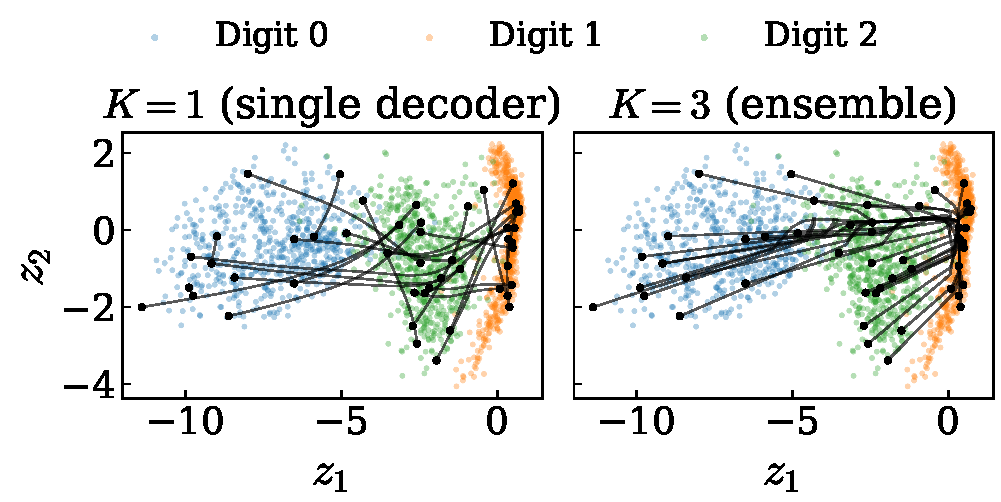
\includegraphics[width=\linewidth]{geodesics.pdf}
    \caption{Geodesics between 25 random latent-variable pairs.
    Left: single decoder ($K{=}1$). Right: ensemble ($K{=}3$).
    Points coloured by digit class.}
    \label{fig:geodesics}
\end{figure}

\subsection*{Part B: Ensemble VAE geometry}

A single decoder's geometry is unreliable: retraining changes $f$ and thus $G$.
We use an ensemble of $K$ independently trained decoders.
The \emph{model-average curve energy} is
\begin{equation}\label{eq:ensemble}
  \mathcal{E}(c) \approx \textstyle\sum_{i=0}^{N} \mathbb{E}_{l,k}\bigl[\|f_l(c(t_i)) - f_k(c(t_{i+1}))\|^2\bigr],
\end{equation}
where $f_l, f_k$ are drawn uniformly and independently from the $K$ decoders (including $l{=}k$).
When $l{\neq}k$, the cross-decoder term penalises decoder \emph{disagreement}, inflating energy in uncertain regions and steering geodesics towards areas where the ensemble is confident.
We approximate~\eqref{eq:ensemble} with $S{=}50$ Monte Carlo $(l,k)$ samples.
Figure~\ref{fig:geodesics} (right) shows ensemble geodesics for the same 25 pairs.

We train $M{=}10$ VAEs and, for each, compute Euclidean and geodesic distances between fixed test-point pairs, encoding with the retrain's own encoder.
The CoV for pair $(i,j)$ is $\text{CoV}_{ij} = \sigma\{d_{ij}^{(m)}\}_{m=1}^{M}\! / \mu\{d_{ij}^{(m)}\}_{m=1}^{M}$, averaged over 10 pairs.
Figure~\ref{fig:cov} shows that Euclidean CoV (0.25) is constant w.r.t.\ $K$, as expected.
Geodesic CoV at $K{=}1$ is lowest (0.20), increases sharply at $K{=}2$ (0.58), then drops to 0.31 at $K{=}3$.
The low $K{=}1$ value reflects that a single decoder yields a deterministic metric per model, so geodesic distances track Euclidean distances closely.
At $K{=}2$, the cross-decoder energy terms ($l{\neq}k$) introduce large variance: with only two decoders and thus a single cross-pair, the magnitude of their disagreement fluctuates strongly across retrainings.
At $K{=}3$, nine $(l,k)$ pairs provide better Monte Carlo coverage and the disagreement averages out, reducing CoV---though not yet below $K{=}1$.
We expect that with larger $K$ the trend would continue downward, and that $M{=}10$ retrainings may be insufficient to resolve the full asymptotic behaviour.

\begin{figure}[H]
    \centering
    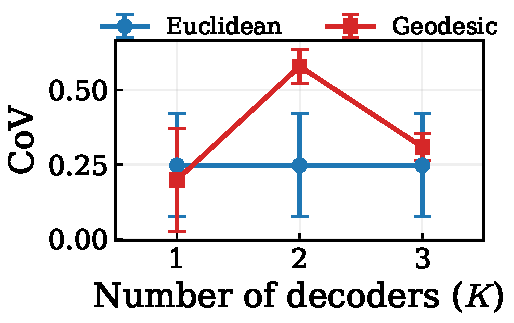
\includegraphics[width=0.75\linewidth]{cov.pdf}
    \caption{Mean CoV ($\pm$1 std) of Euclidean and geodesic distances vs.\ number of ensemble decoders ($M{=}10$ retrainings, 10 pairs).}
    \label{fig:cov}
\end{figure}

\end{multicols}

\newpage

%%% Code snippet part %%%

\section*{Code snippets}

\textbf{Curve energy (Eq.~\ref{eq:energy}).} Decodes all curve points and sums squared output-space differences between consecutive points.
\begin{lstlisting}
def curve_energy(curve_points, decoder):
    decoded = decoder(curve_points).mean          # (N+1, 1, 28, 28)
    decoded_flat = decoded.reshape(len(decoded), -1)  # (N+1, 784)
    diffs = decoded_flat[1:] - decoded_flat[:-1]
    return (diffs ** 2).sum()
\end{lstlisting}

\textbf{Ensemble curve energy (Eq.~\ref{eq:ensemble}).} Pre-decodes with all $K$ decoders, then samples $(l,k)$ pairs uniformly for Monte Carlo estimation.
\begin{lstlisting}
def ensemble_curve_energy(curve_points, decoders, S=50):
    K = len(decoders)
    # Pre-decode all points with all decoders: (K, N+1, D)
    all_dec = torch.stack([d(curve_points).mean.reshape(
                           len(curve_points), -1) for d in decoders])
    l = torch.randint(0, K, (S,))  # MC sample decoder indices
    k = torch.randint(0, K, (S,))
    diffs = all_dec[l, :-1] - all_dec[k, 1:]   # (S, N, D)
    return (diffs ** 2).sum(-1).mean(0).sum()   # avg over S, sum segments
\end{lstlisting}

\textbf{Geodesic computation.} Interior points initialised as linear interpolation, optimised with Adam to minimise curve energy.
\begin{lstlisting}
def compute_geodesic(z0, z1, decoders, T=20, lr=0.01, steps=1000):
    ts = torch.linspace(0, 1, T + 2)[1:-1]
    interior = nn.Parameter(z0 + ts[:, None] * (z1 - z0))  # (T, 2)
    opt = torch.optim.Adam([interior], lr=lr)
    sched = StepLR(opt, step_size=300, gamma=0.5)
    for _ in range(steps):
        opt.zero_grad()
        curve = torch.cat([z0[None], interior, z1[None]])
        energy = ensemble_curve_energy(curve, decoders)
        energy.backward()
        opt.step(); sched.step()
    return torch.cat([z0[None], interior.data, z1[None]])
\end{lstlisting}

\textbf{Coefficient of Variation.} Per-pair CoV across $M$ retrainings, then averaged.
\begin{lstlisting}
# dists: (M, num_pairs) -- geodesic or Euclidean distances
cov_per_pair = dists.std(axis=0) / (dists.mean(axis=0) + 1e-10)
mean_cov = cov_per_pair.mean()  # reported in Figure 2
\end{lstlisting}

\newpage

%%% AI declaration %%%

\section*{Declaration of use of generative AI}

This declaration \textbf{must} be filled out and included as the 3rd page of the document. The questions apply to all parts of the work, including research, project writing, and coding.
\begin{itemize}
\item I/we have used generative AI tools: yes
\end{itemize}
If you answered \emph{yes}, please complete the following sections. List the generative AI tools you have used:
\begin{itemize}
\item Claude (via GitHub Copilot)
\end{itemize}
Describe how the tools were used:
\begin{description}
\item[What did you use the tool(s) for?] Claude was used via GitHub Copilot for code scaffolding (training loops, batch scripts) and \LaTeX{} formatting assistance. All mathematical formulations and experimental design decisions were made by the authors.
\item[At what stage(s) of the process did you use the tool(s)?] During implementation and report writing.
\item[How did you use or incorporate the generated output?] Generated code was reviewed, tested, and modified to fit the project. Report text was drafted by the authors with formatting assistance.
\end{description}

\newpage

%%% References %%%

\section*{References}
All methods and notation follow the materials provided in weeks 5--8 of the Advanced Machine Learning course (02460) at DTU, spring 2026.

\end{document}
